% !TeX spellcheck = en_GB
\begin{figure}[!htb]
  \setlength{\unitlength}{\textwidth}

        \begin{picture}(1,0.4)(-0.02,0)

 
      
      \put(0.08,0.02){\includegraphics[width=0.75\unitlength]{./FnP/surf_pres_tri_10.eps}}

      \put(0.46,0.00){Relativedestance from the leading edge}
      
      
     
       \put(0.1,0.119){\rotatebox{90}{Surface preessure}}
      

      %\put(0.095,0.218){\small(a)}
      %\put(0.565,0.218){\small(b)}
      
    \end{picture}

  \caption{Surface pressure of top ($\times$) and bottom  (\ding{117})surfaces of the static triangular cross section at $10^\circ$. Leading edge of the cross section start from $x=-0.4$. A clear pressure difference is visible between the surfaces. The top surface comparatively has more negative pressure where a lift is created which results in a negative $C_y$}
    \label{fig:surf_press_tri}
\end{figure}

 %vspace{10cm}
